\documentclass[11pt, oneside]{article}   	% use "amsart" instead of "article" for AMSLaTeX format
\usepackage{geometry}                		% See geometry.pdf to learn the layout options. There are lots.
\geometry{letterpaper}                   		% ... or a4paper or a5paper or ... 
%\geometry{landscape}                		% Activate for for rotated page geometry
%\usepackage[parfill]{parskip}    		% Activate to begin paragraphs with an empty line rather than an indent
\usepackage{graphicx}				% Use pdf, png, jpg, or eps� with pdflatex; use eps in DVI mode
								% TeX will automatically convert eps --> pdf in pdflatex		
\usepackage{amssymb}
\usepackage{amsmath}
\usepackage{parskip}
\usepackage{color}
\usepackage{hyperref}

\title{Harmonic Oscillator:  with friction}
%\author{The Author}
%\section{}
%\subsection*{}
\date{}							% Activate to display a given date or no date

\graphicspath{{/Users/telliott_admin/Dropbox/Tex/png/}}
% \begin{center} 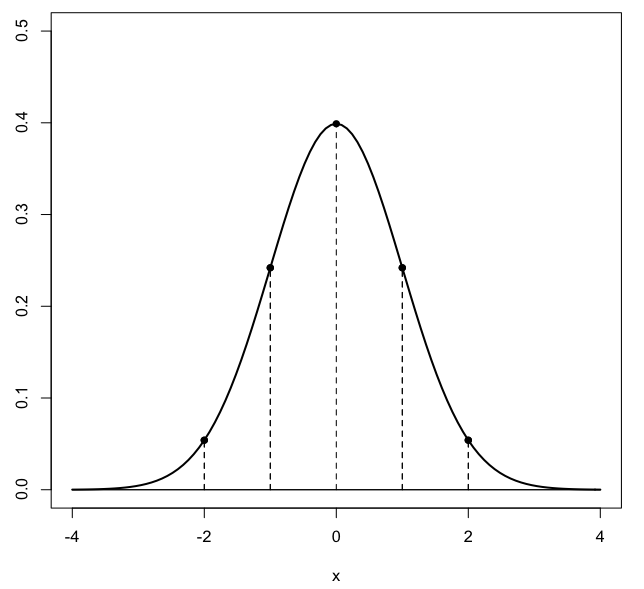
\includegraphics [scale=0.4] {gauss3.png} \end{center}
\begin{document}
\maketitle
\Large
In this short write-up we will add friction to the mass and spring system.
\begin{center} 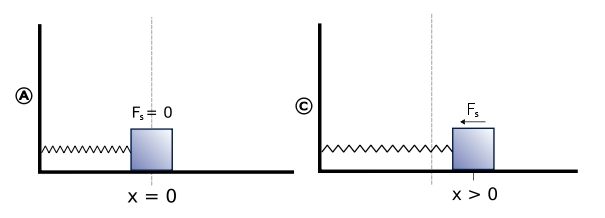
\includegraphics [scale=0.5] {spring1.png} \end{center}
The simple version (no friction) had this equation of motion
\[ \ddot{x} + \omega^2 x = 0 \]
where
\[ \omega^2 = \frac{k}{m} \]
and our solution was
\[ x(t) = A \cos (\omega t + \phi) \]
where $A$ is the amplitude of the oscillation, corresponding to $x(0)$.  The phase $\phi$ allows us to "start the clock" early and have $t=0$ at some later time, where there is a velocity.  Normally, we would not need $\phi$ for the simple example.

We add friction
\[ F = ma = m \ddot{x} = -kx - b \dot{x} \]
\[ m \ddot{x} + b \dot{x} + kx  = 0 \]
Now, the simple cosine function is no longer a solution.

Let's rewrite this as
\[ \ddot{x} + \gamma \dot{x} + \omega^2 x  = 0 \]
where $\gamma = b/m$, and $\omega_0{}^2 = k/m$.  (We've relabeled $\omega$ because there will be more of them soon).

We guess that maybe the exponential is a solution.
\[ x = Ae^{\alpha t} \]
\[ \dot{x} = \alpha Ae^{\alpha t} \]
\[ \ddot{x} = \alpha^2 Ae^{\alpha t} \]
Plugging into the equation of motion we get
\[ [ \ \alpha^2 + \alpha \gamma + \omega_0{}^2 \ ] \ Ae^{\alpha t}  = 0 \]
Now, $A=0$ is a solution, but it's not very interesting.  And fooling with $t$ very large and negative doesn't really help.  The correct approach is to set
\[ \alpha^2 + \alpha \gamma + \omega_0{}^2 = 0 \]
We have converted the differential equation into a quadratic.  Here are two solutions
\[ \alpha = -\frac{\gamma}{2} \pm \sqrt{(\frac{\gamma}{2})^2 - \omega_0{}^2} \]
We will call these two solutions $\alpha_{+}$ and $\alpha_{-}$, according to the sign of the square root term.  We note that not only $\alpha_{-} < 0$ but also $\alpha_{+} \le 0$ as well (ignoring the possibility that $\omega_0{}^2 > (\gamma/2)^2$ for now, see below).

So we write
\[ x(t) = A e^{\alpha_{+}t} + B e^{\alpha_{-}t} \]
These are both falling exponentials, as we would expect.  The motion dies out with time.

$A$ and $B$ will be determined from the initial conditions, $x_0$ and $v_0$.
\[ x_0 = A + B \]
\[ v_0 = \dot{x} = \alpha_{+}A + \alpha_{-}B \]

\subsection*{imaginary exponents}
At this point, it occurs to us that the mass and spring system without friction might also be solved by an exponential.  It can't be a "real" exponential (since we need a stable oscillation).  Instead we will dive into the world of complex exponentials.

The equation of motion was
\[ \ddot{x} + \omega_0{}^2 x = 0 \]
We make a guess
\[ x = A e^{\alpha t} \]
\[ \ddot{x} = \alpha^2 A e^{\alpha t} \]
So we plug in and get
\[ [ \ \alpha^2 + \omega_0{}^2  \ ] \ A e^{\alpha t} \]
The only way this will work is if 
\[ \alpha = \pm \ i \omega_0 \]
We write two solutions
\[ x_1 = A e^{i \omega_0 t} \]
\[ x_2 = B e^{-i \omega_0 t} \]
These work as solutions.
\[ \ddot{x_1} + \omega_0{}^2 x_1 = 0 \]
\[ \ddot{x_2} + \omega_0{}^2 x_2 = 0 \]

The mathematicians are happy, but the physicists are not.  The reason is that $x(t)$ should be real.  The way we get out of this is to add the two solutions together.  Since these are linear equations it works.  It is called the principle of superposition.

Since there are no non-linear terms like $(x_1 + x_2)^2$ or $(\ddot{x}_1 + \ddot{x}_2)^2$, every term is separable as coming from one solution or the other.
\[ x(t) = A e^{i \omega_0 t} + B e^{-i \omega_0 t} \]
If we require in addition that 
\[ B = A^* \]
$B$ is the complex conjugate of $A$, then write
\[ x(t) = A e^{i \omega_0 t} + A^* e^{-i \omega_0 t} \]
Now, it should be clear that the first and second terms are complex conjugates, and therefore, $x(t)$ will be real.

Write 
\[ A = |A|e^{i \phi} \]
\[ A^* = |A|e^{-i \phi} \]
\[ x(t) = |A|e^{i \phi} e^{i \omega_0 t} + |A|e^{-i \phi} e^{-i \omega_0 t} \]
\[ x(t) = |A| \ [ \ e^{i (\omega_0 t + \phi)} + e^{-i (\omega_0 t + \phi)} \ ] \]

Go back to the original work on the complex exponential to recall that
\[ e^{i\theta} = \cos \theta + i \sin \theta \]
\[ e^{-i\theta} = \cos \theta - i \sin \theta \]
\[ e^{i\theta} + e^{-i\theta} = 2\cos \theta \]

What we have above is just
\[ x(t) = 2|A| \cos ( \omega_0 t + \phi ) \]
Define $C = 2|A|$
\[ x(t) = C \cos ( \omega_0 t + \phi ) \]

We got our old answer back again!  In addition to use of Euler's equation, the key is the principle of superposition.

\subsection*{just a little friction}
Up above in the section with friction, we looked at this equation
\[ \alpha^2 + \alpha \gamma + \omega_0{}^2 = 0 \]
\[ \alpha = -\frac{\gamma}{2} \pm \sqrt{(\frac{\gamma}{2})^2 - \omega_0{}^2} \]
We solved it assuming that $\gamma/2 > \omega_0$.  That is, we assumed that friction was large, and the solutions we got reflect that.  Those solutions don't actually oscillate, instead the mass just slowly slides back to rest.

Now we consider other solutions.  Write
\[ \alpha = -\frac{\gamma}{2} \pm i\sqrt{(\omega_0{}^2 - \frac{\gamma}{2})^2} \]
Define
\[ \omega' = \sqrt{(\omega_0{}^2 - \frac{\gamma}{2})^2} \]
\[ \alpha = -\frac{\gamma}{2} \pm i\omega' \]
Our solution becomes
\[ x(t) = A e^{\alpha_{+}t} + B e^{\alpha_{-}t} \]
\[ x(t) = A e^{-\frac{\gamma}{2} + i\omega' t} + B e^{-\frac{\gamma}{2} - i\omega' t} \]
Pull out the common factor
\[ x(t) = e^{-\frac{\gamma}{2}t}(A e^{i\omega' t} + B e^{-i\omega' t}) \]
Use the complex conjugate requirement that we did before to make sure $x$ is real
\[ A = A* \]
\[ x(t) = e^{-\frac{\gamma}{2}t}(A e^{i\omega' t} + A^* e^{-i\omega' t}) \]
\[ = e^{-\frac{\gamma}{2}t} C \cos ( \omega' t + \phi ) \]
Now the solution looks like the cosine, but with an extra exponential part damps it with time.

\subsection*{driven oscillator}
Finally we come to our last problem, the real goal, a harmonic oscillator with a periodic driving force.
\[ \ddot{x} + \gamma \dot{x} + \omega_0{}^2 x = F_0/m \cos \omega t \]
We have enough experience now with the left-hand side to recognize that if we had an exponential on the right we would be in good shape.  Although we don't have that situation, there is a very nice trick!

Make up a new problem.
\[ \ddot{y} + \gamma \dot{y} + \omega_0{}^2 y = F_0/m \sin \omega t \]
Multiply everything by $i$
\[ i\ddot{y} + i\gamma \dot{y} + i\omega_0{}^2 y = i F_0/m \sin \omega t \]
Add it to the problem we really want to solve
\[ \frac{d^2}{dt^2}(x + iy) + \gamma \frac{d}{dt}(x + iy) + \omega_0{}^2 (x + iy) = F_0/m e^{i\omega t} \]
Let's define $z = x + iy$ so
\[ \ddot{z} + \gamma \dot{z} + \omega_0{}^2 z = F_0/m e^{i\omega t} \]

We're going to solve this.  And by the principle of superposition, the real part of the solution will be the solution to the problem (in the real variable $x$) that we started with above.

We guess a solution of the form
\[ z = z_0 \ e^{i \omega t} \]
Taking derivatives and plugging in we get
\[ [ \ -\omega^2 + i \omega \gamma + \omega_0{}^2 \ ] \ z_0 \ e^{i\omega t} = F_0/m \ e^{i\omega t} \]
The expression in brackets is called the impedance.  It is complex.
\[ I = \omega_0{}^2 - \omega^2 + i \omega \gamma \]
We can write 
\[ I = |I| e^{i\phi} \]
Recall that $|x + iy| = \sqrt{x^2 + y^2}$, so to calculate $|I|$ we do
\[ |I| = \sqrt{\omega_0{}^2 - \omega^2)^2 + \omega^2 \gamma^2} \]
furthermore, the angle is the complex part divided by the real part
\[ \phi = tan^{-1} \frac{\omega \gamma}{\omega_0{}^2 - \omega^2} \]
so
\[ I z_0 \ e^{i \omega t} = F_0/m \ e^{i\omega t} \]
\[ z = \frac{F_0/m}{I} \ e^{i\omega t} \]
\[ = \frac{F_0/m}{|I|e^{i\phi}} \ e^{i\omega t}  \]
\[ =  \frac{F_0/m}{|I|} \ e^{i(\omega t - \phi)}\]
Finally, we take the real part as the answer to our problem
\[ x(t) = \frac{F_0/m}{|I|} \ \cos(\omega t - \phi) \]
This solution is called $x_p$ for particular.
\[ x_p = \frac{F_0/m}{|I|} \ \cos(\omega t - \phi) \]
If you're feeling adventurous, you can add the solution to the earlier problem (damped oscillation with friction), which is called $x_c$.
\[ x_c = e^{-\frac{\gamma}{2}t} C \cos ( \omega_0 t + \phi ) \]
$c$ is for complementary.  The final, whole enchilada is
\[ x(t) = x_p + x_c \]
\[ = \frac{F_0/m}{|I|} \ \cos(\omega t - \phi) + e^{-\frac{\gamma}{2}t} C \cos ( \omega_0 t + \phi ) \]
The initial conditions $x_0$ and $v_0$ go into the $x_c$ solution.  However, after some time the system settles down and has forgotten how it started.  Then, only the $x_p$ solution matters.

\end{document}  